\section{Primary results}
    
    From the five specimens used, the model was able to successfully fit all data quite well (total fit $r^2 > 0.97$). Moreover, the final parameter values were quite consistent, with generally low standard errors (table 3). The mean collagen fibre modulus (approx. 279 MPa) and fibre splay (approx. $38^\circ$) were comparable to previous studies \cite{fan_simulation_2014}. Interestingly, the lower bound stretch was small (1.01 or approx. 1\% strain), 
    so it is likely that it could be set to 1 (i.e. zero strain). The native collagen fibre recruitment parameters were also consistent (table 3), and indicated a very rapid recruitment at stretch of approximately 1.18–1.2 (figure \ref{c3:fig:9}). This is a more complete picture of the entire fibre recruitment than in our previous work \cite{sun_finite_2005,fan_simulation_2014}, and suggests that the collagen fibres are effectively well ordered with a small deviation in crimp amplitude and wavelength.
    
    
%%%%%%%%%%%%%%%%%%%%	begin FIGURE 	%%%%%%%%%%%%%%%%%%%%
\begin{figure}
\centering
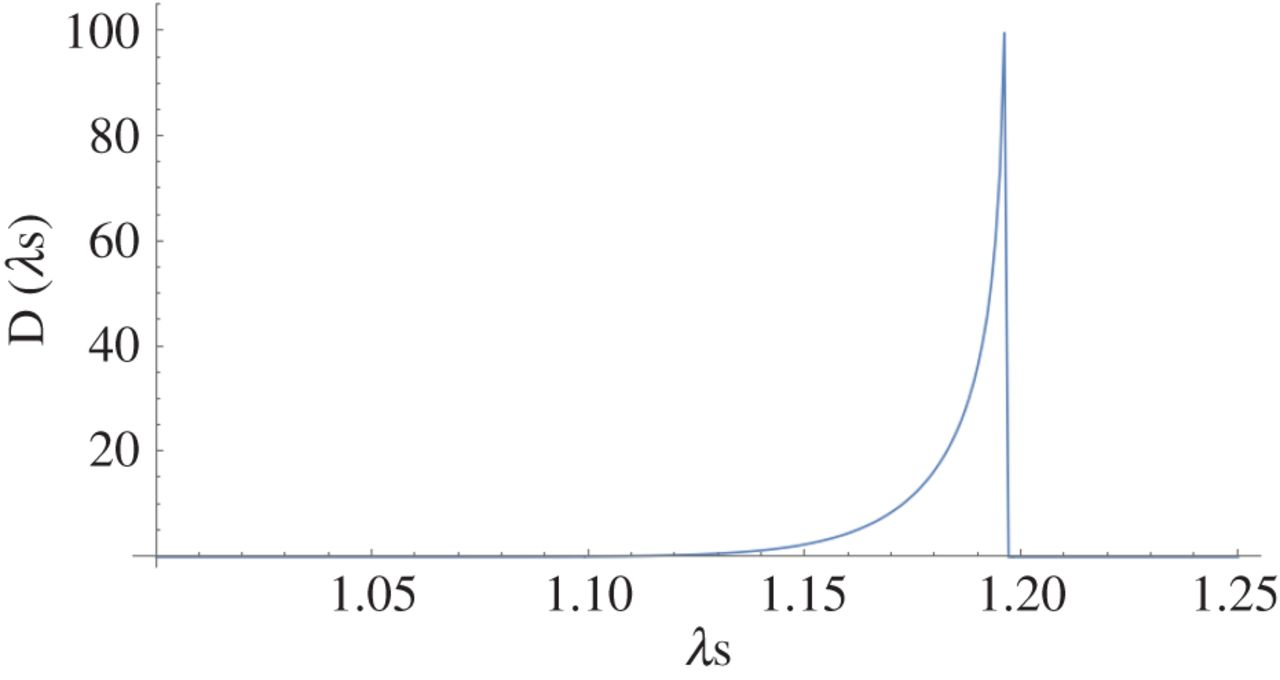
\includegraphics[width=\textwidth]{Images/chapter3/F9large.jpg}
\caption{Representative complete collagen fibre recruitment for the pericardial tissue, showing a rapid recruitment near the upper bound, suggesting the collagen fibres have similar crimp geometries in the native state.}
\label{c3:fig:9}
\end{figure}
%%%%%%%%%%%%%%%%%%%%	 end FIGURE 	%%%%%%%%%%%%%%%%%%%%


\begin{table}
\centering
\caption{Equibiaxial strain testing results.}\label{c3:tab:3}
\begin{tabular}{L{.5in}R{.7in}R{0.5in}R{0.5in}R{0.6in}R{0.5in}R{0.6in}R{0.5in}}
\hline
& \multicolumn{1}{c}{\textbf{modulus}} & \multicolumn{2}{c}{\textbf{ODF}} & \multicolumn{4}{c}{\textbf{recruitment}}\\
\cline{2-8}
& $\eta_c(MPa)$ & $\mu_\Gamma({}^\circ)$ & $\sigma_\Gamma({}^\circ)$ & $\mu_0$ & $\sigma_0$ & $\prescript{}{0}{\lambda}_{lb}$
& $\prescript{}{0}{\lambda}_{ub}$\\
mean & 278.94 & 6.513 & 38.430 & 1.185 & 0.014 & 1.011 & 1.197  \\
s.e.m. & 22.38 & 1.645 & 0.922 & 0.032 & 0.001 & 0.007 & 0.035  \\
\hline
\hline
& \multicolumn{2}{c}{\textbf{Interactions}} & & \multicolumn{4}{c}{\textbf{Matrix}} \\
\cline{2-8}
& $d_0(kPa)$ & $d_1$ & & $\mu_a(kPa)$ & $a$ & $\mu_b(kPa)$ & $b$\\
mean & 1.040 & 42.267 & & 56.74 & 1.068 & 1294.38 & 1.873  \\
s.e.m. & 0.255 & 9.772 & & 10.69 & 0.004 & 340.71 & 0.007 \\
\hline
\end{tabular}
\end{table}


    One advantage of our approach is that the various contributions to the total stress can be separated (figure \ref{c3:fig:8}). To better reveal the present findings, it is useful to examine the effects on the individual stress components under various loading paths. Following the trends of the ensemble results (figure \ref{c3:fig:9}), we noted that the interactions produced substantial contributions to the total stress (figure \ref{c3:fig:10}). Interestingly, for $S_{11}$ the interactions actually produced the largest contributions, followed by the matrix and collagen fibres. By contrast, for $S_{22}$ the contributions were much more dependent on the particular loading path, with the collagen phase dominating when $\lambda_2>\lambda_1$. When $\lambda_1>\lambda_2$, the matrix phase dominated $S_22$. We further note here that the contribution of the matrix was much less loading path sensitive, due to its near-linear, isotropic behaviour.
    
    
    
%%%%%%%%%%%%%%%%%%%%	begin FIGURE 	%%%%%%%%%%%%%%%%%%%%
\begin{figure}
\centering
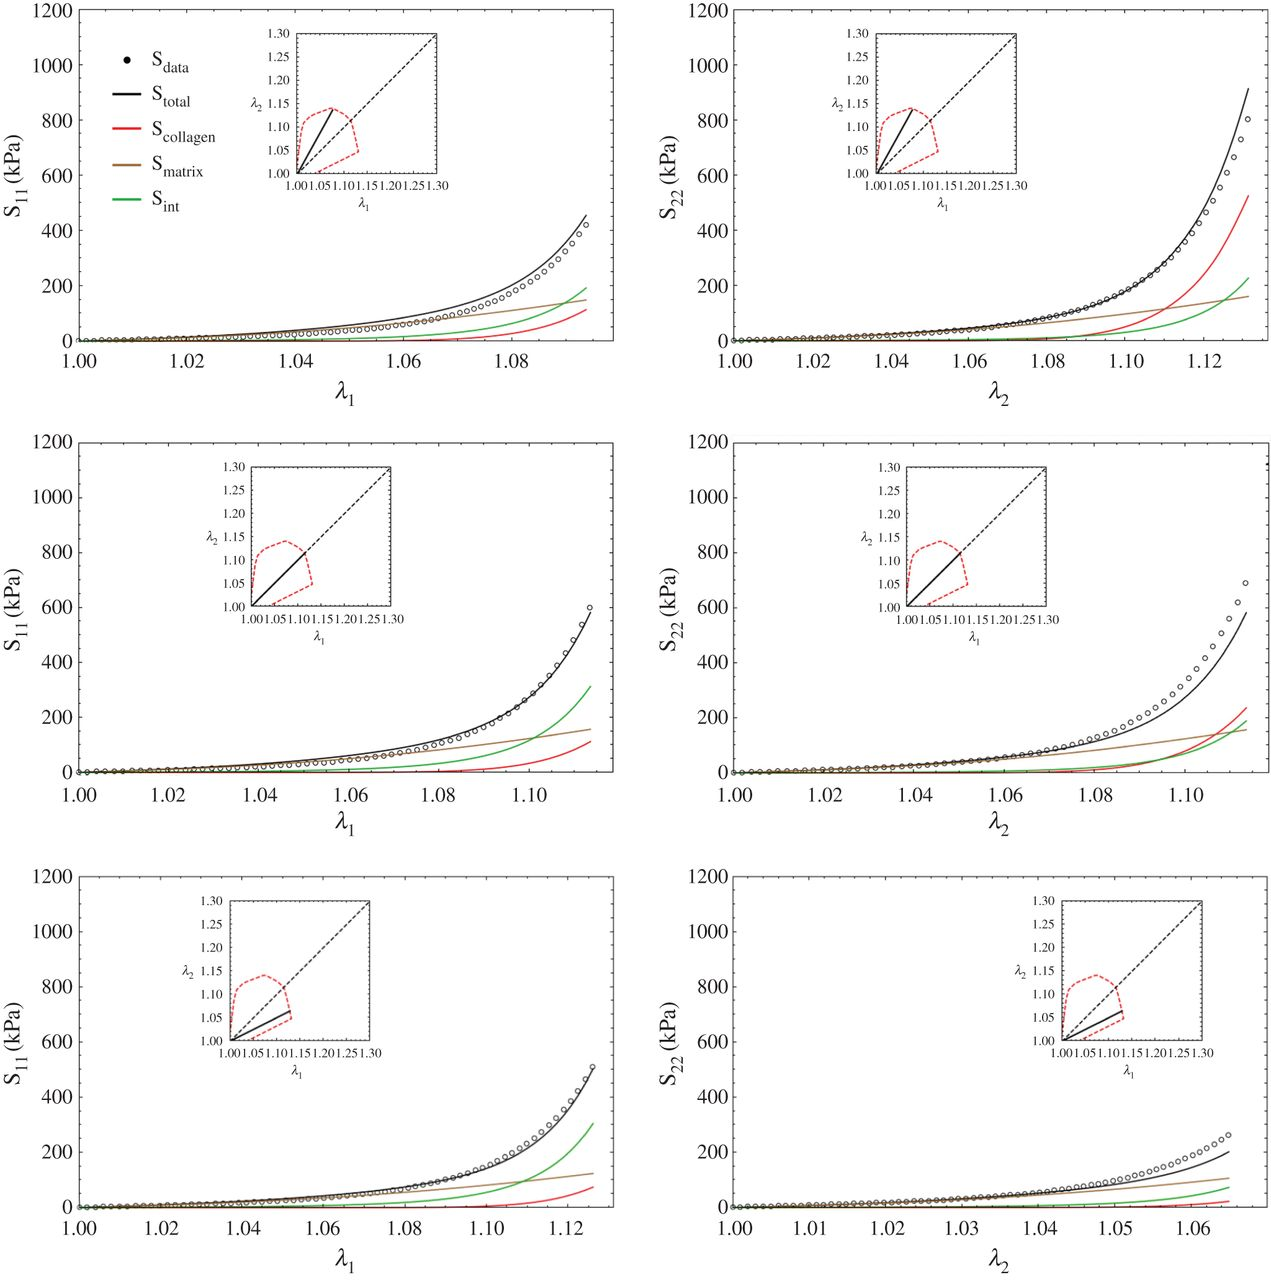
\includegraphics[width=\textwidth]{Images/chapter3/F10large.jpg}
\caption{Complete model (equation \ref{c3:eqn:53}) results for the $S_{11}$ and $S_{22}$ stress components for three protocols. Interestingly for $S_{11}$ the interactions actually produced the largest contributions, followed by the matrix and collagen fibres. By contrast, for $S_{22}$ the contributions were much more dependent on the particular loading path, with the collagen phase dominating when $\lambda_2>\lambda_1$. When $\lambda_1>\lambda_2$ the matrix phase dominated $S_{22}$. We further note here that the contribution of the matrix was much less loading path sensitive, owing to its near-linear, isotropic behaviour.}
\label{c3:fig:10}
\end{figure}
%%%%%%%%%%%%%%%%%%%%	 end FIGURE 	%%%%%%%%%%%%%%%%%%%%